\begin{figure}[H]
    \centering
    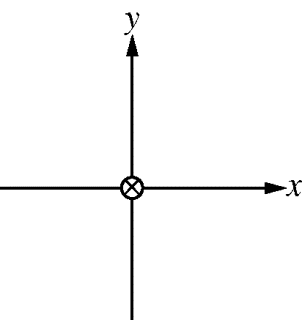
\includegraphics[scale=0.4]{images/img-009-019.png}
\end{figure}

% Multiple Choice Question 21
\begin{questions}\setcounter{question}{20}\question
A long straight wire is located at the origin of an $x y$-coordinate system and is perpendicular to the $x y$-plane. The wire has a current that is directed into the page, as shown in the figure above. Which of the following graphs best represents the magnetic field $\vec{B}$ due to the current as a function of the position $x$ along the $x$-axis? Assume a positive magnetic field to be directed in the $+y$ direction.

\begin{oneparchoices}
\choice \adjustbox{valign=t}{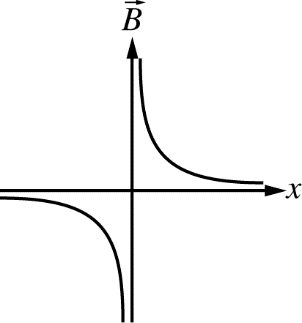
\includegraphics[scale=0.4]{images/img-009-020.png}}
\choice \adjustbox{valign=t}{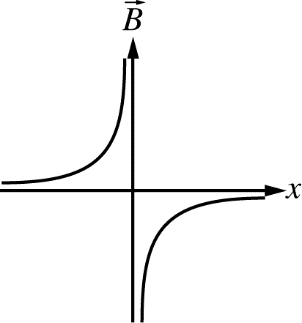
\includegraphics[scale=0.4]{images/img-009-021.png}}
\choice \adjustbox{valign=t}{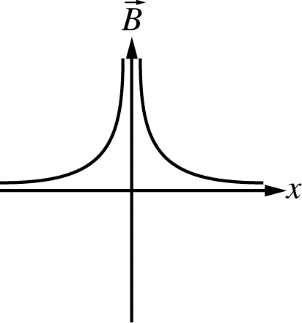
\includegraphics[scale=0.4]{images/img-009-022.png}}
\choice \adjustbox{valign=t}{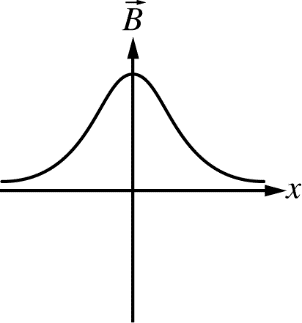
\includegraphics[scale=0.4]{images/img-009-023.png}}
\choice \adjustbox{valign=t}{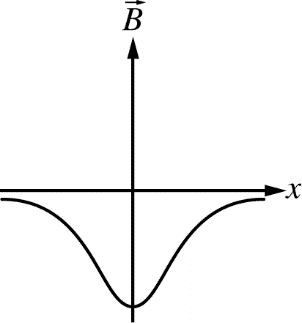
\includegraphics[scale=0.4]{images/img-009-024.png}}
\end{oneparchoices}\end{questions}
